\documentclass[serif]{beamer}
%\usepackage[utopia]{mathdesign}
%\usepackage[no-math]{fontspec}
%\setmainfont{Liberation Serif}

\usepackage{minted}
% \usepackage{redhat}
\usepackage{hyperref}
\usepackage{ccicons}

\usepackage{tikz}
\usetikzlibrary{arrows,shapes,snakes,automata,backgrounds,petri}

\title{How fuzzing helps to find bugs}
\author{Zbigniew Jędrzejewski-Szmek}
\institute{%
  \includegraphics{beamer-themeredhat/redhat.png}\\
  \medskip
  \textit{zbyszek@in.waw.pl}\\
  \medskip
  \ccbysa
}
\date{\tiny Brno, 25.1.2019}

\begin{document}
\begin{frame}
\titlepage % Print the title page as the first slide
\end{frame}

\begin{frame}
  \frametitle{Why?}

  Various tools to write C/C++/Fortan
  \begin{itemize}
  \item compiler diagnostics
  \item static analysis (coverity, LGTM, ..., clang-analyzer)
  \item unit tests
  \item asserts
  \item \emph{fuzzing}
  \end{itemize}

  \bigskip
  
  \tiny
  Good for any project in a compiled language.\\
  General principle applies to incremented or safe languages, but this talk is about C/C++.
\end{frame}

\begin{frame}
    tl;dr: fuzzing finds \emph{different} errors than other tools
\end{frame}

\begin{frame}
  \frametitle{How?}

  \emph{Fuzzing engines}
  take care of providing nice varied inputs \\
  → fuzzing

  \medskip

  \tiny
  The number of possible code paths is exponential, so simply testing
  all combinations of bytes is not useful.

  A feedback loop from runtime code coverage to input generation
  allows better coverage compared to blind variation
\end{frame}

\begin{frame}
  \frametitle{Modern fuzzing}

  \begin{itemize}
  \item code instrumentation to provide coverage information
  \item genetic algorithms to generate useful paths
  \end{itemize}

\end{frame}

\begin{frame}[fragile]
  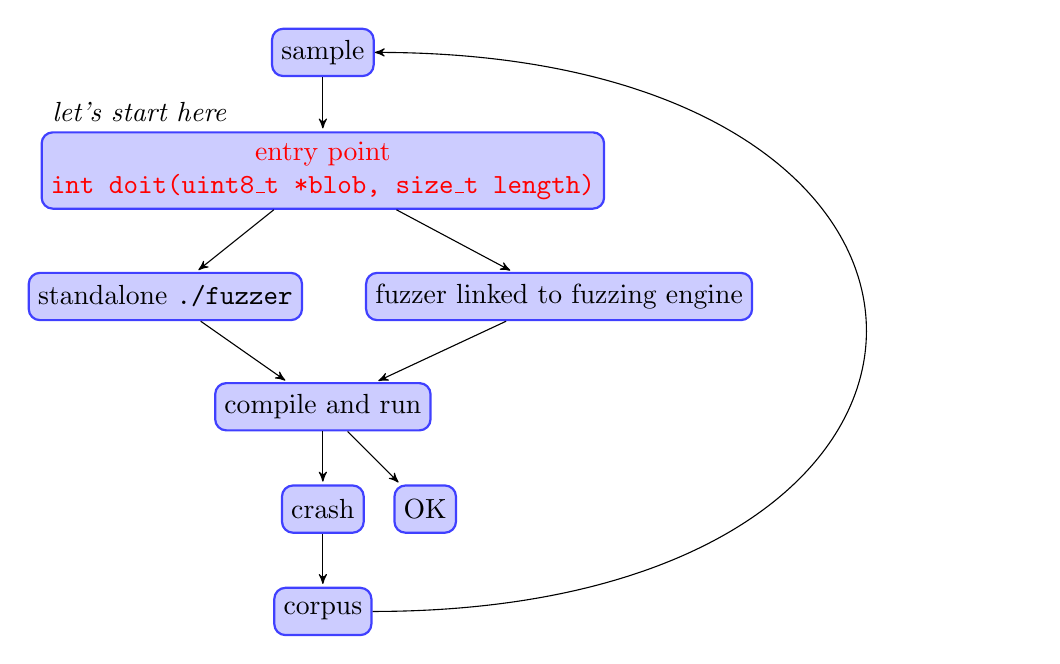
\begin{tikzpicture}[node distance=1.3cm,>=stealth',bend angle=45,auto]
    \tikzstyle{place}=[rectangle,thick,draw=blue!75,fill=blue!20,minimum size=6mm, rounded corners]

    \begin{scope}
      \node [place] at (0, +1.5) (sample) {sample};

      \node [place, text=red, align=center] (entry)  [label=above:\emph{let's start here}\phantom{xxxxxxxxxxxxxxxxxxxxxxxxx}] {entry point\\ \texttt{int doit(uint8\_t *blob, size\_t length)}}
        edge [pre] (sample);

      \node [place] at (-2, -1.6) (standalone)      {standalone \texttt{./fuzzer}}
        edge [pre] (entry);
      \node [place] at (+3, -1.6) (lib)          {fuzzer linked to fuzzing engine}
        edge [pre] (entry);

      \node [place] at (0, -3)    (run)         {compile and run}
        edge [pre] (standalone)
        edge [pre] (lib);
      \node [place] (crash) [below of=run]                 {crash}
        edge [pre] (run);
      \node [place] (OK) [right of=crash]                 {OK}
        edge [pre] (run);
      \node [place] (corpus) [below of=crash]            {corpus}
        edge [pre] (crash);

        % \draw [->] (crash) to[out=-280,in=-180,looseness=4] (standalone);
       \draw [->] (corpus) to[out=-0,in=0,looseness=3] (sample);

    \end{scope}

  \end{tikzpicture}
\end{frame}

\begin{frame}
  \frametitle{Checking}

  Normal checking mechanisms are used:
  \begin{itemize}
  \item AddressSanitizer
  \item MemorySanitizer
  \item LeakSanitizer
  \item valgrind
  \item asserts
  \item any checks built into the code, e.g. malloc/free checks
  \end{itemize}

  \pause
  We want to crash as \emph{soon} as possible!
\end{frame}

\begin{frame}
  \frametitle{What bugs can we find}

  \begin{itemize}
  \item buffer overflows
  \item crashes on input
  \item double free\\[1 em]

  \item use-after-free
  \item buffer overreads\\[1 em]

  \item infinite loops
  \item resource exhaustion: oom, quadratic loops
  \end{itemize}
\end{frame}

\begin{frame}
  \frametitle{Coverage feedback}

  \begin{itemize}
  \item SanitizerCoverage (libfuzzer)
  \end{itemize}
\end{frame}

\begin{frame}
  \frametitle{In-process vs. out-of-process}

  \begin{itemize}
  \item each sample should run quickly (< 100 ms)
  \item no global state, threads, or persistence
  \item we can avoid the overhead of process spawning
  \end{itemize}
\end{frame}

\begin{frame}
  \frametitle{Fuzzing engines}
  \begin{itemize}
  \item (standalone)
  \item libfuzzer
  \item AFL
  \item honggfuzz
  \item radamsa
  \end{itemize}

  Most fuzzing engines provide an easy way to do in-process testing.

  \pause
  Now we just need a lot of cores to run the code over many many input samples.
\end{frame}

\begin{frame}
  \frametitle{oss-fuzz}

  A service for open source projects to do continuous fuzzing

  \bigskip

  \pause
  oss-fuzz:
  \begin{itemize}
  \item run the fuzzers with all configured sanitizers
  \item report bugs privately
  \item close bugs automatically once a fix is committed
  \item do regression tests for old bugs
  \item make bugs public after a delay
  \end{itemize}
\end{frame}

\begin{frame}
  \frametitle{Adding oss-fuzz support to a project}

  \begin{columns}
    \begin{column}[t]{0.5\textwidth}
      In the project\\
      → entry points\\
      → \texttt{fuzzers} target to build the fuzzers
    \end{column}
    \begin{column}[t]{0.5\textwidth}
      In oss-fuzz.git\\
      → project metainfo in \texttt{project.yaml}\\
      → \texttt{Dockerfile} to prepare the build environment\\
      → \texttt{build.sh} to call the \texttt{fuzzers} target
    \end{column}
  \end{columns}
\end{frame}

\begin{frame}[fragile]
  \frametitle{Example: casync}

  \begin{minted}{C}
int LLVMFuzzerTestOneInput(const uint8_t *data,
                           size_t size) {
        ...

        return 0;
}
\end{minted}
\end{frame}

\begin{frame}[fragile]
\small
  \begin{minted}{C}
typedef struct header {
        uint32_t alg;
        uint32_t reserved[5];
        uint8_t data[];
} header;

int LLVMFuzzerTestOneInput(const uint8_t *data, size_t size) {
        if (size < offsetof(header, data) + 1)
                return 0;

        const header *h = (struct header*) data;
        const size_t data_len = size - offsetof(header, data);

        if (h->reserved[0] || h->reserved[1] || h->reserved[2]
            || h->reserved[3] || h->reserved[4])
                return 0;

        ...

        return 0;
}
\end{minted}
\end{frame}

\begin{frame}[fragile]
\small
  \begin{minted}{C}
typedef struct header {
        uint32_t alg;
        uint32_t reserved[5];
        uint8_t data[];
} header;

int LLVMFuzzerTestOneInput(const uint8_t *data, size_t size) {
        if (!getenv("CASYNC_LOG_LEVEL"))
                set_log_level(LOG_CRIT);

        if (size < offsetof(header, data) + 1)
                return 0;

        const header *h = (struct header*) data;
        const size_t data_len = size - offsetof(header, data);

        if (h->reserved[0] || h->reserved[1] || h->reserved[2]
            || h->reserved[3] || h->reserved[4])
                return 0;

        ...

        return 0;
}
\end{minted}
\end{frame}

\begin{frame}[fragile]
\small
  \begin{minted}{C}
int LLVMFuzzerTestOneInput(const uint8_t *data, size_t size) {
        ...
        CompressorContext c = COMPRESSOR_CONTEXT_INIT;

        r = compressor_start_decode(&c, h->alg);
        if (r < 0)
                return log_debug_errno(r, "compressor_start_decode failed: %m");

        log_info("Using compression %d, data size=%zu", h->alg, data_len);

        size_t out_size = MAX(size, 128u), ret_done;
        buf = malloc(out_size);
        if (!buf)
                return log_oom();

        r = compressor_decode(&c, buf, out_size, &ret_done);
        if (r < 0)
                return log_debug_errno(r, "compressor_decode failed: %m");
        return 0;
}
\end{minted}
\end{frame}

\begin{frame}[fragile]
\small
\begin{minted}{Docker}
# projects/casync/Dockerfile    
FROM gcr.io/oss-fuzz-base/base-builder
MAINTAINER zbyszek@in.waw.pl
RUN apt-get update && \
    apt-get install -y python3-pip pkg-config wget \
        liblzma-dev libzstd-dev libcurl4-openssl-dev \
        libssl-dev libudev-dev zlib1g-dev libacl1-dev \
        libfuse-dev rsync udev python3-sphinx && \
    pip3 install meson ninja
RUN git clone --depth 1 https://github.com/systemd/casync casync
WORKDIR casync
COPY build.sh $SRC/
\end{minted}

\begin{minted}{yaml}
# projects/casync/project.yaml
homepage: "https://github.com/casync/casync"
sanitizers:
  - address
  - undefined
  - memory
auto_ccs:
  - zbyszek@in.waw.pl
  - poettering@gmail.com
\end{minted}
\end{frame}

\begin{frame}[fragile]
  \frametitle{Running the fuzzers}
  
  \begin{minted}{bash}
sudo ...
python infra/helper.py build_image casync
python infra/helper.py build_fuzzers casync ~/src/casync
python infra/helper.py run_fuzzer casync fuzz-compress
  \end{minted}
\end{frame}

\begin{frame}[fragile]
  \tiny
  \begin{minted}{console}
$ sudo python infra/helper.py run_fuzzer casync fuzz-compress
  \end{minted}
  \begin{minted}{text}
Running: docker run --rm -i --privileged -e FUZZING_ENGINE=libfuzzer -e SANITIZER=address -e RUN_FUZZER_MODE=interactive -v /home/zbyszek/src/fuzz/oss-fuzz/build/out/casync:/out -t gcr.io/oss-fuzz-base/base-runner run_fuzzer fuzz-compress
/out/fuzz-compress -rss_limit_mb=2048 -timeout=25 < /dev/null
INFO: Seed: 2775442882
INFO: Loaded 1 modules   (596 inline 8-bit counters): 596 [0x8c9aa8, 0x8c9cfc), 
INFO: Loaded 1 PC tables (596 PCs): 596 [0x8c9d00,0x8cc240), 
INFO: -max_len is not provided; libFuzzer will not generate inputs larger than 4096 bytes
INFO: A corpus is not provided, starting from an empty corpus
#2	INITED cov: 3 ft: 4 corp: 1/1b lim: 4 exec/s: 0 rss: 27Mb
	NEW_FUNC[1/6]: 0x536130 in compressor_start_decode /work/build/../../src/casync/src/compressor.c:44
	NEW_FUNC[2/6]: 0x5364e0 in compressor_finish /work/build/../../src/casync/src/compressor.c:145
#2454	NEW    cov: 15 ft: 17 corp: 2/26b lim: 25 exec/s: 0 rss: 28Mb L: 25/25 MS: 2 InsertRepeatedBytes-CopyPart-
#2518	NEW    cov: 16 ft: 18 corp: 3/51b lim: 25 exec/s: 0 rss: 29Mb L: 25/25 MS: 4 CopyPart-CrossOver-ChangeBit-InsertRepeatedBytes-
	NEW_FUNC[1/3]: 0x5366a0 in compressor_input /work/build/../../src/casync/src/compressor.c:182
	NEW_FUNC[2/3]: 0x536870 in compressor_decode /work/build/../../src/casync/src/compressor.c:219
#3366	NEW    cov: 27 ft: 29 corp: 4/77b lim: 33 exec/s: 0 rss: 29Mb L: 26/26 MS: 3 ChangeByte-InsertByte-ChangeBinInt-
#3479	NEW    cov: 32 ft: 38 corp: 5/103b lim: 33 exec/s: 0 rss: 29Mb L: 26/26 MS: 3 ShuffleBytes-ChangeByte-ChangeBit-
#3539	NEW    cov: 33 ft: 39 corp: 6/131b lim: 33 exec/s: 0 rss: 29Mb L: 28/28 MS: 5 ChangeBinInt-InsertRepeatedBytes-EraseBytes-ChangeBit-ChangeBinInt-
#3685	REDUCE cov: 33 ft: 39 corp: 6/128b lim: 33 exec/s: 0 rss: 29Mb L: 25/26 MS: 1 EraseBytes-
#3941	NEW    cov: 34 ft: 40 corp: 7/153b lim: 33 exec/s: 0 rss: 29Mb L: 25/26 MS: 1 CMP- DE: "\x01\x00\x00\x00\x00\x00\x00\x19"-
#4549	NEW    cov: 35 ft: 41 corp: 8/191b lim: 38 exec/s: 0 rss: 31Mb L: 38/38 MS: 3 ChangeByte-ChangeBit-InsertRepeatedBytes-
#4920	REDUCE cov: 35 ft: 41 corp: 8/189b lim: 38 exec/s: 0 rss: 31Mb L: 36/36 MS: 1 EraseBytes-
#5622	REDUCE cov: 35 ft: 41 corp: 8/188b lim: 43 exec/s: 0 rss: 32Mb L: 25/36 MS: 2 CrossOver-EraseBytes-
#14903	REDUCE cov: 36 ft: 42 corp: 9/323b lim: 135 exec/s: 0 rss: 43Mb L: 135/135 MS: 1 CrossOver-
#15734	REDUCE cov: 36 ft: 42 corp: 9/319b lim: 142 exec/s: 0 rss: 43Mb L: 131/131 MS: 1 EraseBytes-
#15893	REDUCE cov: 36 ft: 42 corp: 9/318b lim: 142 exec/s: 0 rss: 43Mb L: 130/130 MS: 4 ChangeBinInt-CopyPart-ChangeBinInt-EraseBytes-
#17009	REDUCE cov: 36 ft: 42 corp: 9/317b lim: 149 exec/s: 0 rss: 44Mb L: 129/129 MS: 1 EraseBytes-
#131072	pulse  cov: 36 ft: 42 corp: 9/317b lim: 1280 exec/s: 65536 rss: 52Mb
#262144	pulse  cov: 36 ft: 42 corp: 9/317b lim: 2578 exec/s: 65536 rss: 56Mb
#524288	pulse  cov: 36 ft: 42 corp: 9/317b lim: 4096 exec/s: 58254 rss: 61Mb
#1048576	pulse  cov: 36 ft: 42 corp: 9/317b lim: 4096 exec/s: 61680 rss: 61Mb
#2097152	pulse  cov: 36 ft: 42 corp: 9/317b lim: 4096 exec/s: 59918 rss: 61Mb
\end{minted}
\end{frame}

\begin{frame}[fragile]
  \tiny
  \begin{minted}{console}
$ sudo python infra/helper.py run_fuzzer casync fuzz-compress
  \end{minted}
  \begin{minted}{text}
#2254	NEW    cov: 16 ft: 18 corp: 3/51b lim: 25 exec/s: 0 rss: 29Mb L: 25/25 MS: 3 ChangeBit-EraseBytes-CopyPart-
=================================================================
==10==ERROR: AddressSanitizer: heap-buffer-overflow on address 0x6030000042e9 at pc 0x000000456979 bp 0x7fff5debce50 sp 0x7fff5debc600
READ of size 2 at 0x6030000042e9 thread T0
SCARINESS: 14 (2-byte-read-heap-buffer-overflow)
    #0 0x456978 in __interceptor_memcpy.part.38 /src/llvm/projects/compiler-rt/lib/asan/../sanitizer_common/sanitizer_common_interceptors.inc:802
    #1 0x7f74ed62e30c  (/lib/x86_64-linux-gnu/liblzma.so.5+0x230c)
    #2 0x7f74ed634b9d  (/lib/x86_64-linux-gnu/liblzma.so.5+0x8b9d)
    #3 0x7f74ed62e5e5 in lzma_code (/lib/x86_64-linux-gnu/liblzma.so.5+0x25e5)
    #4 0x536b0c in compressor_decode /work/build/../../src/casync/src/compressor.c:243:23
    #5 0x535d8d in LLVMFuzzerTestOneInput /work/build/../../src/casync/test/fuzz/fuzz-compress.c:57:13
    #6 0x56a675 in fuzzer::Fuzzer::ExecuteCallback(unsigned char const*, unsigned long) /src/libfuzzer/FuzzerLoop.cpp:532:15
    #7 0x568c42 in fuzzer::Fuzzer::RunOne(unsigned char const*, unsigned long, bool, fuzzer::InputInfo*, bool*) /src/libfuzzer/FuzzerLoop.cpp:454:3
    #8 0x56c122 in fuzzer::Fuzzer::MutateAndTestOne() /src/libfuzzer/FuzzerLoop.cpp:669:19
    #9 0x56f096 in fuzzer::Fuzzer::Loop(std::__1::vector<std::__1::basic_string<char, std::__1::char_traits<char>, std::__1::allocator<char> >, fuzzer::fuzzer_allocator<std::__1::basic_string<char, std::__1::char_traits<char>, std::__1::allocator<char> > > > const&) /src/libfuzzer/FuzzerLoop.cpp:800:5
    #10 0x54ccb7 in fuzzer::FuzzerDriver(int*, char***, int (*)(unsigned char const*, unsigned long)) /src/libfuzzer/FuzzerDriver.cpp:764:6
    #11 0x53fcec in main /src/libfuzzer/FuzzerMain.cpp:19:10
    #12 0x7f74ec52082f in __libc_start_main (/lib/x86_64-linux-gnu/libc.so.6+0x2082f)
    #13 0x41dae8 in _start (/out/fuzz-compress+0x41dae8)

0x6030000042e9 is located 0 bytes to the right of 25-byte region [0x6030000042d0,0x6030000042e9)
allocated by thread T0 here:
    #0 0x531798 in operator new[](unsigned long) /src/llvm/projects/compiler-rt/lib/asan/asan_new_delete.cc:109
    #1 0x56a427 in fuzzer::Fuzzer::ExecuteCallback(unsigned char const*, unsigned long) /src/libfuzzer/FuzzerLoop.cpp:519:23
    #2 0x568c42 in fuzzer::Fuzzer::RunOne(unsigned char const*, unsigned long, bool, fuzzer::InputInfo*, bool*) /src/libfuzzer/FuzzerLoop.cpp:454:3
    #3 0x56c122 in fuzzer::Fuzzer::MutateAndTestOne() /src/libfuzzer/FuzzerLoop.cpp:669:19
    #4 0x56f096 in fuzzer::Fuzzer::Loop(std::__1::vector<std::__1::basic_string<char, std::__1::char_traits<char>, std::__1::allocator<char> >, fuzzer::fuzzer_allocator<std::__1::basic_string<char, std::__1::char_traits<char>, std::__1::allocator<char> > > > const&) /src/libfuzzer/FuzzerLoop.cpp:800:5
    #5 0x54ccb7 in fuzzer::FuzzerDriver(int*, char***, int (*)(unsigned char const*, unsigned long)) /src/libfuzzer/FuzzerDriver.cpp:764:6
    #6 0x53fcec in main /src/libfuzzer/FuzzerMain.cpp:19:10
    #7 0x7f74ec52082f in __libc_start_main (/lib/x86_64-linux-gnu/libc.so.6+0x2082f)
\end{minted}
\end{frame}

\begin{frame}[fragile]
  \tiny
  ...
  \begin{minted}{text}
SUMMARY: AddressSanitizer: heap-buffer-overflow /src/llvm/projects/compiler-rt/lib/asan/../sanitizer_common/sanitizer_common_interceptors.inc:802 in __interceptor_memcpy.part.38
Shadow bytes around the buggy address:
  0x0c067fff8840: fa fa fd fd fd fd fa fa fd fd fd fd fa fa fd fd
=>0x0c067fff8850: fd fd fa fa fd fd fd fd fa fa 00 00 00[01]fa fa
  0x0c067fff8860: fa fa fa fa fa fa fa fa fa fa fa fa fa fa fa fa
Shadow byte legend (one shadow byte represents 8 application bytes):
  Addressable:           00
  Partially addressable: 01 02 03 04 05 06 07 
  Heap left redzone:       fa
  Freed heap region:       fd
  Stack left redzone:      f1
  Stack mid redzone:       f2
  Stack right redzone:     f3
  Stack after return:      f5
  Stack use after scope:   f8
  Global redzone:          f9
  Global init order:       f6
  Poisoned by user:        f7
  Container overflow:      fc
  Array cookie:            ac
  Intra object redzone:    bb
  ASan internal:           fe
  Left alloca redzone:     ca
  Right alloca redzone:    cb
  Shadow gap:              cc
==10==ABORTING
MS: 4 ShuffleBytes-ChangeBinInt-ChangeByte-ChangeBinInt-; base unit: f49b78e08a2abefbdf6b63fd66d001431483d041
0x0,0x0,0x0,0x0,0x0,0x0,0x0,0x19,0xd4,0x38,0x0,0xd4,0x0,0x0,0x0,0x0,0x0,0x0,0x0,0xd4,0xd4,0xd4,0x41,0xd4,0xd4,
\x00\x00\x00\x00\x00\x00\x00\x19\xd48\x00\xd4\x00\x00\x00\x00\x00\x00\x00\xd4\xd4\xd4A\xd4\xd4
artifact_prefix='./'; Test unit written to ./crash-297edd631777b45e87a73eb0ebe8e81f76da25cb
  \end{minted}
\end{frame}

\begin{frame}[fragile]
  \frametitle{Links}

  \url{https://github.com/systemd/casync}\\
  {\small
    \href{https://bugs.chromium.org/p/oss-fuzz/issues/list?can=1&q=type=Bug-Security,Bug%20-component:Infra%20status:Fixed,Verified&sort=-id&colspec=ID%20Type%20Component%20Status%20Library%20Reported%20Owner%20Summary}{https://bugs.chromium.org/p/oss-fuzz/issues/list?type=Bug-Security...}\hspace*{-2cm}
  }\\

  \url{https://oss-fuzz.com}\\
    
  \url{https://github.com/google/fuzzer-test-suite/blob/master/tutorial/libFuzzerTutorial.md}\\

  \url{http://llvm.org/docs/LibFuzzer.html}

\end{frame}

\end{document}
